\documentclass[xcolor={dvipsnames}]{beamer}
\usepackage{color, colortbl}
\usepackage[ngerman,english]{babel}
\usepackage[T1]{fontenc}
\usepackage{lmodern}
\usepackage[compatibility=false]{caption}
\usepackage{subcaption}
\usepackage{tikz}
\usepackage{textgreek}
\usepackage{tabularx}
\usepackage{booktabs}
\usepackage{siunitx}
\usepackage{appendixnumberbeamer}
\usepackage[absolute,overlay]{textpos} %for positioning the logos where I want

\usepackage{animate}
\usepackage{multimedia}
\usepackage{fixltx2e}
\usepackage{multicol}
\usepackage{comment}
\DeclareSIUnit\year{yr}

\mode<presentation>
{
  \usetheme{CambridgeUS}     
  \usecolortheme{lily} 
  \definecolor{beamer@violet}{rgb}{0.5,0.3,0.5} % changed this
  \setbeamercolor{structure}{fg=beamer@violet!70!cyan}
  \setbeamercolor{palette primary}{fg=black, bg=gray!30!white!50!cyan!20!}
  \setbeamercolor{palette secondary}{fg=black, bg=gray!30!white!30!cyan!40!}
  \setbeamercolor*{palette tertiary}{bg=gray!20!white!20!cyan!60!}
  
  \setbeamercolor{frametitle}{fg=cyan!60!white!40!,bg=cyan!80!black}
  \setbeamercolor{title}{fg=cyan!80!black}
  \setbeamercolor{normal text}{fg=black,bg=white}
  \setbeamercolor{alerted text}{fg=beamer@violet}
  \setbeamercolor{example text}{fg=beamer@violet!70!cyan}
  
  \usefonttheme{structureitalicserif} 
  \setbeamertemplate{navigation symbols}{}
  \setbeamertemplate{caption}[numbered]
}
\newcommand{\sidlogo}{
  \setlength{\TPHorizModule}{1pt}
  \setlength{\TPVertModule}{1pt}
   % textblock{}{x,y}: pos(x) = rightUpperCorner + (x * \TPHorizModule), pos(y) = leftUpperCorner - (y * \TPVertModule)
  \begin{textblock}{1}(323,12)
   
\includegraphics[width=40pt,height=26pt]{figures/SiD.jpeg}
  \end{textblock}
  } 
\newcommand{\ilclogo}{
  \setlength{\TPHorizModule}{1pt}
  \setlength{\TPVertModule}{1pt}
   % textblock{}{x,y}: pos(x) = rightUpperCorner + (x * \TPHorizModule), pos(y) = leftUpperCorner - (y * \TPVertModule)
  \begin{textblock}{1}(323,12)
   
\includegraphics[width=40pt,height=26pt]{figures/ILC.jpeg}
  \end{textblock}
} 
\newcommand{\flukalogo}{
  \setlength{\TPHorizModule}{1pt}
  \setlength{\TPVertModule}{1pt}
   % textblock{}{x,y}: pos(x) = rightUpperCorner + (x * \TPHorizModule), pos(y) = leftUpperCorner - (y * \TPVertModule)
  \begin{textblock}{1}(315,12)
   
\includegraphics[width=60pt,height=26pt]{figures/fluka_logo.png}
  \end{textblock}
} 

\title[Neutrons from the main beam dumps]{\textbf{\alert{AWLC 2017} \\ \vspace*{0.3cm} The International Linear Collider \\ \LARGE Neutrons from the main beam dumps}}
\author{\textbf{Anne Sch\"utz}}
\institute{\textbf{DESY}}
\date{\textbf{26. June 2017}}

\titlegraphic{
\includegraphics[height=1.0cm]{figures/ILC.jpeg}\hspace*{6cm}~%
   
\includegraphics[height=1.2cm]{figures/DESY_Logo.png}
}

\begin{document}

{
\usebackgroundtemplate{
 \tikz\node[opacity=0.1]{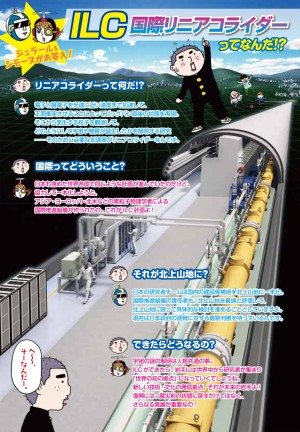
\includegraphics[width=\paperwidth]{figures/Iwatecomics.jpg}};
 % \tikz\node[opacity=0.2]{\centering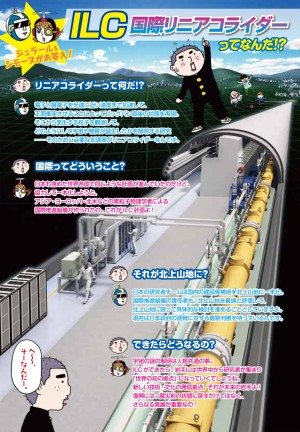
\includegraphics[height=\paperheight]{figures/Iwatecomics.jpg}};
 }
\begin{frame}
  \titlepage
\end{frame}
}

\begin{frame}{Table of contents}
  \tableofcontents
\end{frame}



\section{FLUKA simulation of the ILC Beam Dump}
\subsection{Project Overview}
{
\usebackgroundtemplate{
\vbox to \paperheight{\vfil
 \tikz\node[opacity=0.1]{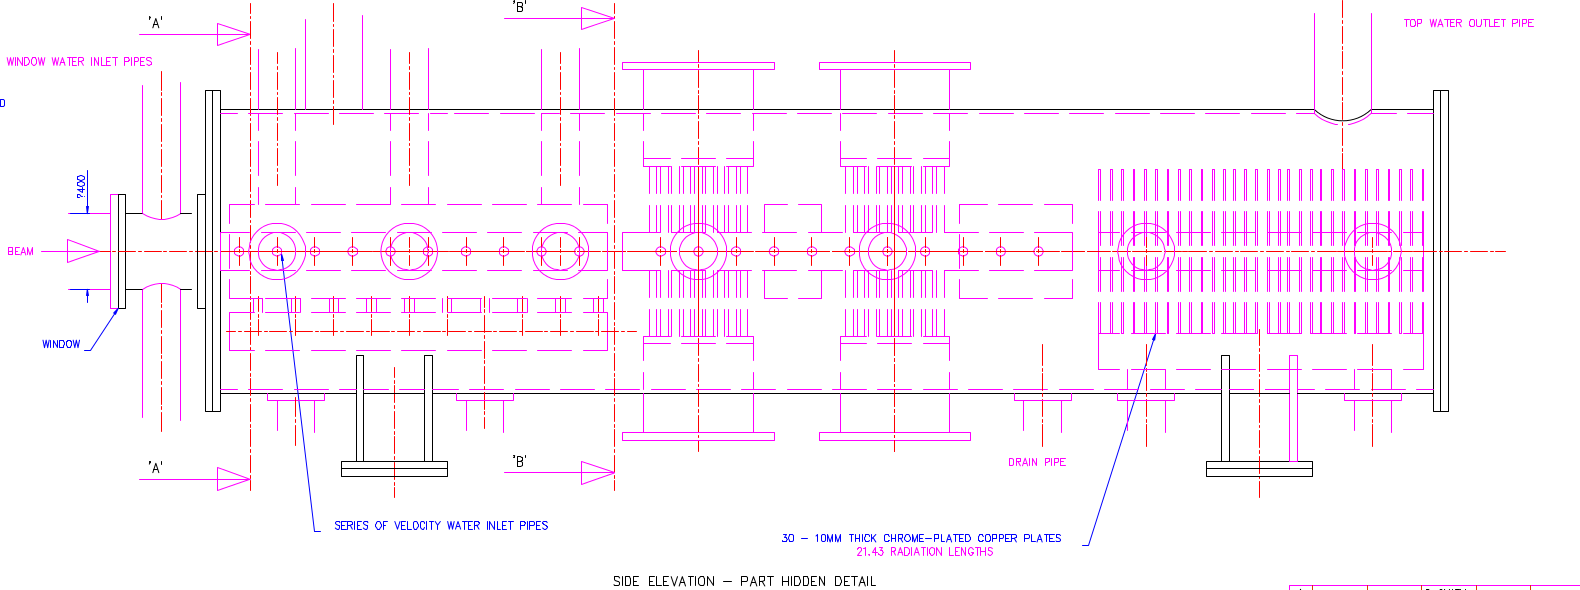
\includegraphics[width=\paperwidth]{figures/TB-0067-300-00-A_yz_view.png}};
 \vfil}
}
\begin{frame}{Neutron Background and Beam Dump Irradiation}
\flukalogo
The 17\,MW\footnote{13.7\,MW average beam power + 20\% margin} beam is dumped into a water tank after collision.\\Neutrons ($\lesssim$\SI{e10}{\per\square\centi\metre\per\year}) are emitted that radiate the surroundings, and travel back towards the detectors.\\
\vspace*{0.1cm}
\alert{Simulating the energy depostions, irradiation, and number of background particles:}
\begin{enumerate}
 \item Simulating the neutrons from the beam dump with FLUKA, using the design drawings by B. Smith~\cite{Smith} to model the dump and the surrounding.
 \item With Benno List (DESY): Python program to plug the real extraction line lattice into FLUKA.\\
Realistic simulation of the interaction between the neutrons and the lattice.
 \item Simulating the neutrons reaching the interaction point in a full detector simulation.
\end{enumerate}
\end{frame}
}

\AtBeginSubsection[] {
  \begin{frame}<beamer>
     \tableofcontents[currentsection,
     currentsubsection,
     %hideothersubsections,
     subsectionstyle=show/shaded/hide,
     subsubsectionstyle=show/show/hide]
  \end{frame}
}

\subsection{The Beam Dump Designs}
\begin{frame}{Designs by B. Smith}
Design drawings by B. Smith, 2006-2007~\cite{Smith}:
\begin{itemize}
 \item two different desings for the water beam dump: 0-TB-0067-210-00-A, 0-TB-0067-300-00-A
 \item shielding walls: 0-TB-0067-404-00-A
 \item surface site: 0-TB-0067-410-00-A
\end{itemize}
Report ``18\,MW Water Beam Dump Design''~\cite{Smith_Report} about considerations and studies of:
\begin{itemize}
 \item Material qualities
 \item Water temperature and pressure
 \item Technical specifications of the dump designs
\end{itemize}
\end{frame}

\begin{frame}{\textbf{Surface site}: 0-TB-0067-410-00-A}
\centering
\only<1>{
  \includegraphics[width=0.9\textwidth]{figures/0067_404-House.png}
 }
 \only<2>{
   \includegraphics[height=0.92\textheight]{figures/0067_404-House_zoom.png}
 }
\end{frame}
\begin{frame}{\textbf{Shielding walls}: 0-TB-0067-404-00-A}
\centering
\only<1>{
 \includegraphics[width=0.92\textwidth]{figures/0067_404-Shielding.png}
 }
 \only<2>{
  \includegraphics[width=0.65\textwidth,angle=90]{figures/0067_404-Shielding_zoom.png}
  }
\end{frame}

\begin{frame}{\textbf{Design 1}: 0-TB-0067-210-00-A}
\centering
 \includegraphics[width=0.92\textwidth]{figures/TB-0067-210-00-A.png}
\end{frame}
{
\usebackgroundtemplate{
\vbox to \paperheight{\vspace*{1.2cm}
 \tikz\node[opacity=0.3]{\hspace*{0.6cm} \includegraphics[width=0.92\textwidth]{figures/TB-0067-210-00-A.png}};
 \vfil}}
\begin{frame}{\textbf{Design 1}: 0-TB-0067-210-00-A}
\begin{columns}
 \begin{column}{0.5\textwidth}
  Vessel:
  \begin{itemize}
   \item Diameter: 1.5\,m
   \item Length: 6.5\,m
   \item 316L Stainless Steel
   \item Water pressure: 10\,bar
  \end{itemize}
  Window:
  \begin{itemize}
   \item Diameter: 300\,mm
   \item Thickness: 1\,mm
   \item Titanium alloy: Ti-6Al-4V 
  \end{itemize}
 \end{column}
 \begin{column}{0.5\textwidth}
  27\,X\textsubscript{0} needed to stop a 500\,GeV beam:
  \begin{itemize}
   \item Water: 18\,X\textsubscript{0}
   \item Water cooled copper plates: 9\,X\textsubscript{0} = 126\,mm
  \end{itemize}  
 \end{column}
\end{columns}

\end{frame}
}
\begin{frame}{\textbf{Design 1}: 0-TB-0067-210-00-A}
\centering
 \includegraphics[width=\textwidth]{figures/Design1_geometry.png}
\end{frame}
\begin{frame}{\textbf{Design 1}: 0-TB-0067-210-00-A}
\centering
 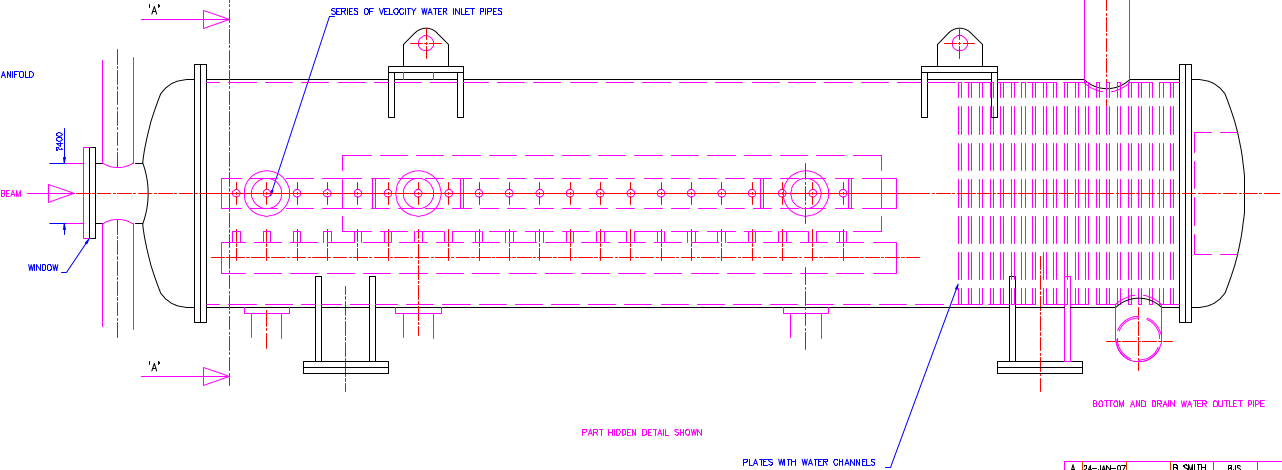
\includegraphics[width=0.5\textwidth]{figures/TB-0067-210-00-A_yz_view.png}
 \hfill
 \includegraphics[width=0.48\textwidth]{figures/Design1_geometry_3Dinside.png}
\end{frame}

\begin{frame}{\textbf{Design 2}: 0-TB-0067-300-00-A}
\centering
  \includegraphics[width=0.92\textwidth]{figures/TB-0067-300-00-A.png}
\end{frame}
{
\usebackgroundtemplate{
\vbox to \paperheight{\vspace*{1.2cm}
 \tikz\node[opacity=0.3]{\hspace*{0.6cm} \includegraphics[width=0.92\textwidth]{figures/TB-0067-300-00-A.png}};
 \vfil}}
\begin{frame}{\textbf{Design 2}: 0-TB-0067-210-00-A}
\begin{columns}
 \begin{column}{0.5\textwidth}
  Vessel:
  \begin{itemize}
   \item Diameter: 1.5\,m
   \item Length: 6.5\,m
   \item 316L Stainless Steel
   \item Water pressure: 10\,bar
  \end{itemize}
  Window:
  \begin{itemize}
   \item Diameter: 300\,mm
   \item Thickness: 1\,mm
   \item Titanium alloy: Ti-6Al-4V 
  \end{itemize}
 \end{column}
 \begin{column}{0.5\textwidth}
  27\,X\textsubscript{0} needed to stop a 500\,GeV beam:
  \begin{itemize}
   \item Water: 18\,X\textsubscript{0}
   \item Water cooled copper plates: 9\,X\textsubscript{0} = 126\,mm
  \end{itemize}  
    Additionally high water pressure section:
  \begin{itemize}
   \item Titanium tubes
   \item High pressure water flow
  \end{itemize} 
 \end{column}
\end{columns}

\end{frame}
}
\begin{frame}{\textbf{Design 2}: 0-TB-0067-300-00-A}
\centering
  \includegraphics[width=\textwidth]{figures/Design2_geometry.png}
\end{frame}
\begin{frame}{\textbf{Design 2}: 0-TB-0067-300-00-A}
\centering
  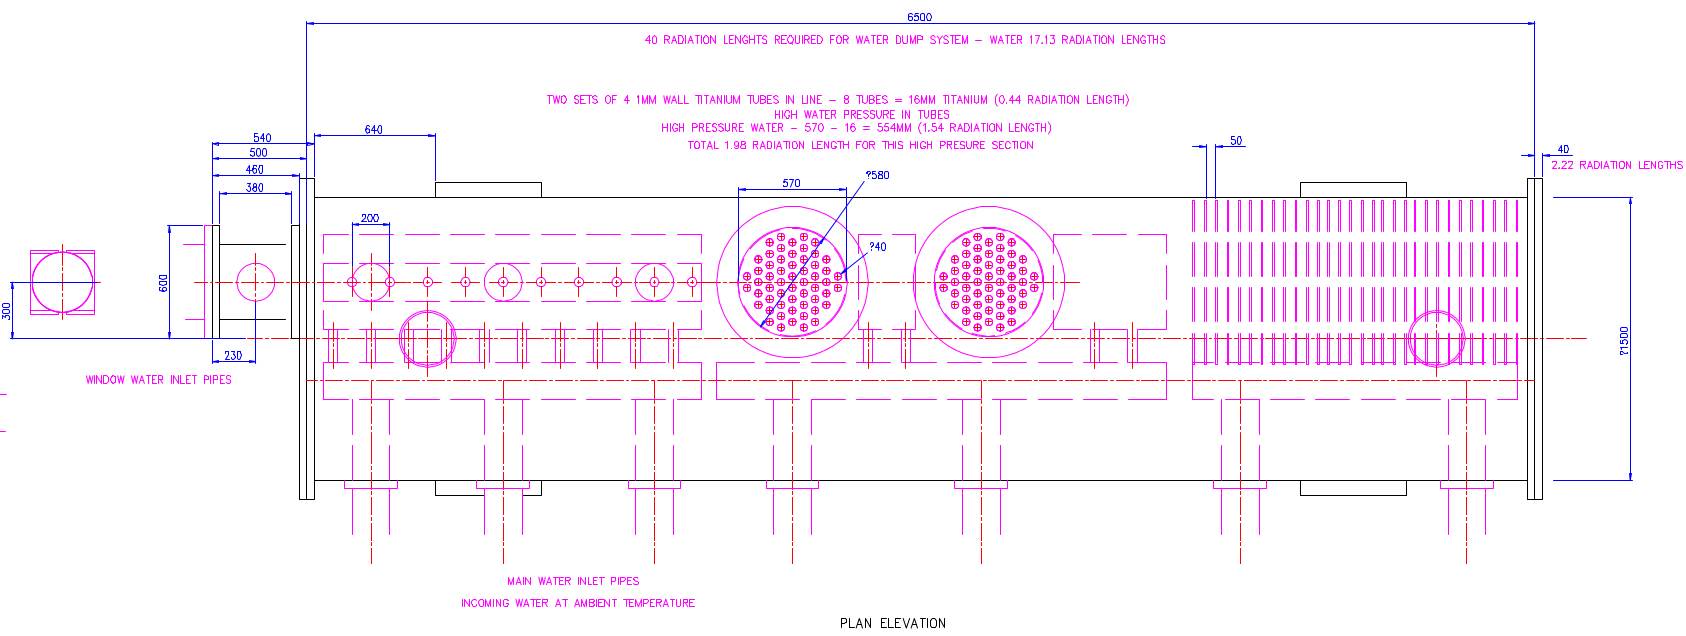
\includegraphics[width=0.5\textwidth]{figures/TB-0067-300-00-A_xz_view.png}
  \hfill
  \includegraphics[width=0.48\textwidth]{figures/Design2_geometry_drawing_xz.png}
\end{frame}
\begin{frame}{\textbf{Design 2}: 0-TB-0067-300-00-A}
\centering
  \includegraphics[width=0.49\textwidth]{figures/Design2_geometry_3Dinside1.png}
    \includegraphics[width=0.49\textwidth]{figures/Design2_geometry_3Dinside2.png}\\
      \includegraphics[width=0.49\textwidth]{figures/Design2_geometry_3Dinside3.png}
\end{frame}



\subsection{The FLUKA simulation}
\begin{frame}
 ILC1000B:
 \begin{itemize}
  \item Beam energy: 500\,GeV
  \item Bunch population: 1.74e10
  \item Bunch size: \textsigma\textsubscript{x} = 2.4\,mm, \textsigma\textsubscript{y} = 0.22\,mm
  \item Bunches per train: 2450
  \item Bunch train duration: 896.7\,\textmu s
 \end{itemize}

\end{frame}


\subsubsection{Deposited Energy and Dose}
\begin{frame}{Deposited Energy}
\centering
\hspace*{1.6cm} Design 1 \hfill Design 2 \hspace*{1.8cm} \\
  \includegraphics[width=0.52\textwidth]{figures/Energy_deposition_xz_Design1.pdf}
    \includegraphics[width=0.52\textwidth]{figures/Energy_deposition_xz_Design1.pdf}
\end{frame}
\begin{frame}{Deposited Engery over Z}
\centering
\hspace*{1.6cm} Design 1 \hfill Design 2 \hspace*{1.8cm} \\
  \includegraphics[width=0.52\textwidth]{figures/Dose_equivalent_total_1DMax_z_Design1.pdf}
    \includegraphics[width=0.52\textwidth]{figures/Dose_equivalent_total_1DMax_z_Design2.pdf}
\end{frame}
%\begin{frame}{Total dose and EM dose}
%\centering
%  \includegraphics[width=0.52\textwidth]{figures/Dose.pdf}
%  \includegraphics[width=0.52\textwidth]{figures/Dose_EM.pdf}
%\end{frame}
\begin{frame}{Dose equivalent after cooling times}
  \begin{center}
  \animategraphics[loop,width=0.49\textwidth]{0.5}{DoseEQ_Time/Design1_}{1}{5}
  \animategraphics[loop,width=0.49\textwidth]{0.5}{DoseEQ_Time/Design2_}{1}{5}
  \end{center}
\end{frame}
\begin{frame}
  \frametitle{Dose equivalent after cooling times}
  \hypertarget{coolingtimesprev}{}
  \centering
    \hspace*{1.6cm} Instantanuous \hfill After 1 minute \hfill After 1 hour \hspace*{1.8cm} \\
  \hyperlink{Dose_equivalent}{\includegraphics[width=0.3\textwidth]{figures/Dose_equivalent_total_Design1.pdf}}
  \includegraphics[width=0.3\textwidth]{DoseEQ_Time/Design1_1.pdf}
  \includegraphics[width=0.3\textwidth]{DoseEQ_Time/Design1_2.pdf}\\
    \hspace*{1.6cm} After 1 day \hfill After 1 month \hfill After 1 year\hspace*{1.8cm} \\
  \includegraphics[width=0.3\textwidth]{DoseEQ_Time/Design1_3.pdf}
  \includegraphics[width=0.3\textwidth]{DoseEQ_Time/Design1_4.pdf}
  \includegraphics[width=0.3\textwidth]{DoseEQ_Time/Design1_5.pdf}
\end{frame}

\begin{frame}{Dose Equivalent over Z}
\centering
\hspace*{1.6cm} Design 1 \hfill Design 2 \hspace*{1.8cm} \\
  \includegraphics[width=0.52\textwidth]{figures/Dose_equivalent_total_1DMax_z_Design1.pdf}
    \includegraphics[width=0.52\textwidth]{figures/Dose_equivalent_total_1DMax_z_Design2.pdf}
\end{frame}

\AtBeginSubsubsection[] {
  \begin{frame}<beamer>
     \tableofcontents[currentsection,
     currentsubsection,
     %hideothersubsections,
     subsectionstyle=show/shaded/hide,
     subsubsectionstyle=show/show/hide]
  \end{frame}
}

\subsubsection{Residual nuclei}
\begin{frame}{Residual nuclei after cooling times}
\centering
\hspace*{1.6cm} Instantanuous \hfill After 1 minute \hspace*{1.8cm} \\
  \includegraphics[width=0.52\textwidth]{figures/Residual_nuclei_Design1.pdf}
  \includegraphics[width=0.52\textwidth]{figures/Residual_nuclei_1minute_Design1.pdf}
\end{frame}
\begin{frame}{Residual nuclei after cooling times}
\centering
\hspace*{1.6cm} After 1 hour \hfill After 1 day \hspace*{1.8cm} \\
  \includegraphics[width=0.52\textwidth]{figures/Residual_nuclei_1hour_Design1.pdf}
  \includegraphics[width=0.52\textwidth]{figures/Residual_nuclei_1day_Design1.pdf}
\end{frame}
\begin{frame}{Residual nuclei after cooling times}
\centering
\hspace*{1.6cm} After 1 month \hfill After 1 year \hspace*{1.8cm} \\
  \includegraphics[width=0.52\textwidth]{figures/Residual_nuclei_1month_Design1.pdf}
  \includegraphics[width=0.52\textwidth]{figures/Residual_nuclei_1year_Design1.pdf}
\end{frame}

\subsubsection{Tritium}
\begin{frame}{Tritium fluxes}
\centering
  \includegraphics[width=0.52\textwidth]{figures/Tritium_flux_xz_Design1.pdf}
\end{frame}

\subsubsection{Particle Fluxes}
\begin{frame}{Proton and Photon fluxes}
\centering
\hspace*{2cm} Protons \hfill Photon \hspace*{2cm} \\
  \includegraphics[width=0.52\textwidth]{figures/Proton_flux_xz_Design1.pdf}
  \includegraphics[width=0.52\textwidth]{figures/Photon_flux_xz_Design1.pdf}
\end{frame}
\begin{frame}{Electron and Positron fluxes}
\centering
\hspace*{2cm} Electrons \hfill Positrons \hspace*{2cm} \\
  \includegraphics[width=0.52\textwidth]{figures/Electron_flux_xz_Design1.pdf}
  \includegraphics[width=0.52\textwidth]{figures/Electron_flux_xz_Design1.pdf}
\end{frame}
\begin{frame}{Neutron fluxes}
\centering
  \includegraphics[width=0.52\textwidth]{figures/Neutron_flux_xz_Design1.pdf}\\
  \centering
\hspace*{1.6cm} x-direction \hfill y-direction \hfill z-direction \hspace*{1.8cm} \\
  \includegraphics[width=0.3\textwidth]{figures/Neutron_flux_1DMax_x_Design1.pdf}
  \includegraphics[width=0.3\textwidth]{figures/Neutron_flux_1DMax_y_Design1.pdf}
  \includegraphics[width=0.3\textwidth]{figures/Neutron_flux_1DMax_z_Design1.pdf}
\end{frame}
\begin{frame}{Neutron fluxes}
\centering
  \includegraphics[width=0.52\textwidth]{figures/Neutron_distribution_WaterTankEnd1_0-90_Design1.pdf}
\end{frame}



\section{Summary and Outlook}
\begin{frame}{Summary and outlook}
 \flukalogo
 Aspects already addressed:
\begin{itemize}
 \item The number of neutrons produced,
 \item the dose of the beam dump surrounding,
 \item the influence of the water composition (amount of deuterium),
 \item the influence of the steel composition of the tank container,
 \item the amount of tritium produced in the water,
 \item the effect of the beam dump design.
\end{itemize}
\vspace*{0.2cm}
 Goals for the next months:
\begin{itemize}
 \item Simulating the neutron flux through the EXT line,
 \item the number of neutrons reaching the IP,
 \item the neutron occupancy in SiD.
\end{itemize}
\end{frame}


\section*{The end}
{
\usebackgroundtemplate{
 \tikz\node[opacity=0.1]{\includegraphics[width=\paperwidth,resolution=200]{figures/ilc-Comic.png}};
 % \tikz\node[opacity=0.2]{\centering\includegraphics[height=\paperheight]{figures/Iwatecomics.jpg}};
 }
\begin{frame}
\ilclogo
\begin{center}
\textcolor{RubineRed}{
	\LARGE Thanks!\\
}
\end{center}
\end{frame}
}

\section*{References}
\begin{thebibliography}{9}
\begin{frame}{References}
\setbeamertemplate{bibliography item}[text]
\bibitem{Smith} B. Smith (Rutherford Lab), \emph{Design drawings 0-TB-0067-300-00-A, 0-TB-0067-210-00-A, 0-TB-0067-404-00-A}, Dec. 2006 - Jan. 2007
\bibitem{TDR} T. Behnke, et al.
\emph{The International Linear Collider - Technical Design Report}, 2013.
\bibitem{LHC TDR} \emph{LHC - Design Report}, \url{http://ab-div.web.cern.ch/ab-div/Publications/LHC-DesignReport.html}
\bibitem{IP beam parameters} ATLAS-CONF-2010-027. \emph{Characterization of Interaction-Point Beam Parameters Using the pp Event-Vertex Distribution Reconstructed in the ATLAS Detector at the LHC}, 2010. \url{http://cds.cern.ch/record/1277659/files/ATLAS-CONF-2010-027.pdf}
\end{frame}
\end{thebibliography}

%--------------------------------------------------------------------------------
\appendix

\begin{frame}
\begin{center}
\LARGE Additional Material
\end{center}
  \tableofcontents
\end{frame}

\section{ILC}

%------Definition for column color in table
\definecolor{Gray}{gray}{0.9}
\newcolumntype{g}{>{\columncolor{Gray}}r}
%-----------------------------------------
\subsection{The ILC beam parameters}
\begin{frame}{The beam parameters of the ILC compared to LHC}
\ilclogo

\begin{table}[]
\centering
\begin{tabularx}{\textwidth}{ll|rrrg}
\hline
& & \multicolumn{1}{>{\centering}p{1.5cm}}{\textbf{Baseline 500}} & \multicolumn{1}{>{\centering}p{1.5cm}}{\textbf{Lumi Upgrade}} & \multicolumn{1}{>{\centering}p{1.5cm}}{\textbf{TeV Upgrade}} & {\centering\textbf{LHC 25ns}} \\ 
\hline
\cline{1-6}
\hline
E$_{CM}$  &[\si{\GeV}] & 500  & 500  & \num{1000} & \num{14000}\\
n$_b$ & & \num{1312} & \num{2625} & \num{2450} &  \num{2808} \\
$\Delta t_b$ &[\si{\nano\second}] & 554  & 366   & 366 & 25 \\
N & & \num{2.0e10}  & \num{2.0e10}  & \num{1.74e10}  & \num{11.5e10}\\
q$_b$ &[\si{\nano\coulomb}] & 3.2  & 3.2  &  2.7 & 18.4 \\
$\sigma_x^*$ &[\si{\nano\metre}] & 474  & 474  &  481 & \num{16700}\\
$\sigma_y^*$ &[\si{\nano\metre}] & 5.9 &  5.9  &  2.8 & \num{16700}\\
$\sigma_z$ &[\si{\milli\metre}] & 0.3  &  0.3  &  0.25 & 0.755\\
L &[\si{\per\centi\metre\squared\per\second}] & \num{1.8e34} & \num{3.6e34} & \num{3.6e34} & \num{1.0e34}\\
\hline
\end{tabularx}
\end{table}
\end{frame}

\begin{frame}{ILC baseline parameters}
\ilclogo
\centering
	\includegraphics[width=\textwidth]{figures/ILCTDR-VOLUME_3-PART_II_ILCparameters.pdf}
\end{frame}
\begin{frame}{ILC parameters for the different upgrade stages}
\ilclogo
\centering
	\includegraphics[width=0.8\textwidth]{figures/ILCTDR-VOLUME_3-PART_II_ILCparametersUpgrades.pdf}
\end{frame}

\section{Zoom Plots}
\begin{frame}
  \begin{center}
    \huge
    ZOOM PLOTS\\
    \tiny
    Here be dragons
  \end{center}
\end{frame}
\begin{frame}[plain]
 \hypertarget{Dose_equivalent}{\hyperlink{coolingtimesprev}{\includegraphics[width=\textwidth]{figures/Dose_equivalent_total_Design1.pdf}}}
\end{frame}


\end{document}
